\chapter{Theoretischer Teil} \label{theorie}

\section{Einleitung} \label{theorieeinleitung}
Ein Spektrum besteht aus 2051 Zahlenwerten. Im Fall der FieldSpec 3 und 4 Spektrometer wird dieses Spektrum noch in drei Teile unterteilt. \gls{vnir}, \gls{swir1} und \gls{swir2}.

\section{Messverfahren} \label{messverfahren}
Das Spektrometer misst die Werte immer im gleichen Verfahren. Als R�ckgabe vom Ger�t wird immer die gleiche Datenstruktur verarbeitet. Diese ist unter genauer beschrieben. Damit sp�ter die drei Verfahren angewendet und in Dateien abgespeichert werden k�nnen m�ssen einige Referenz-Werte vorg�ngig vorhanden sein. Diese Werden zum Teil ebenfalls direkt mit dem Spektrometer erfasst, wie eine White Reference oder Dark Current. Referenz-Werte f�r die Radiance-Berechnung sprich die Base, Lamp und FiberOptic Datei werden beim Konfigurieren des Spektrometers in die App importiert und abgespeichert.

\subsection{Abspeichern vs. Anzeigen}
Die berechneten Daten der Reflectance und Radiance werden in der App \textbf{nur} angezeigt aber niemals in eine Datei geschrieben. Die Daten die in den Messdateien abgespeichert werden sind immer Raw Daten. In den Messdateien sind somit alle Daten vorhanden um sp�ter wieder eine Reflectance oder Radiance Berechnung durchzuf�hren.

\begin{figure}[h]
	\begin{center}
		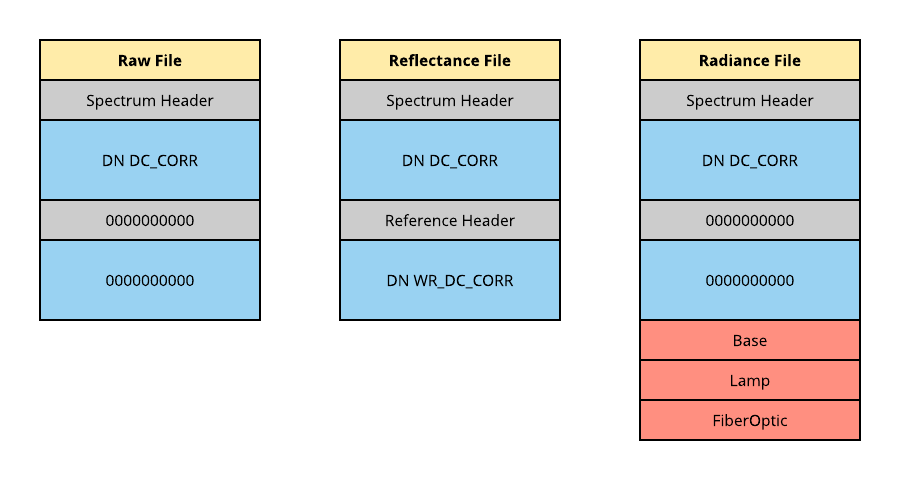
\includegraphics[scale=0.35]{images/IndicoFileFormats} 
	\caption{Inhalt der Messdateien}
	\label{fig:MeasurementFiles}
	\end{center}
\end{figure}

\section{Berechnungsablauf} \label{berechnungsablauf}
Im unterstehenden Diagramm wird der Messablauf grafisch dargestellt. An der blauen Linie ist zu erkennen, dass wiederum nur \gls{dndccorr} und \gls{dnwrdccorr} in die Messdateien geschrieben wird. Die berechneten Werte von Reflectance und Radiance werden nur f�r die Diagramm-Anzeige im App verwendet. Auf die genauen Berechnungen wird im n�chsten Kapitel genauer hingewiesen.

\begin{figure}[h]
	\begin{center}
		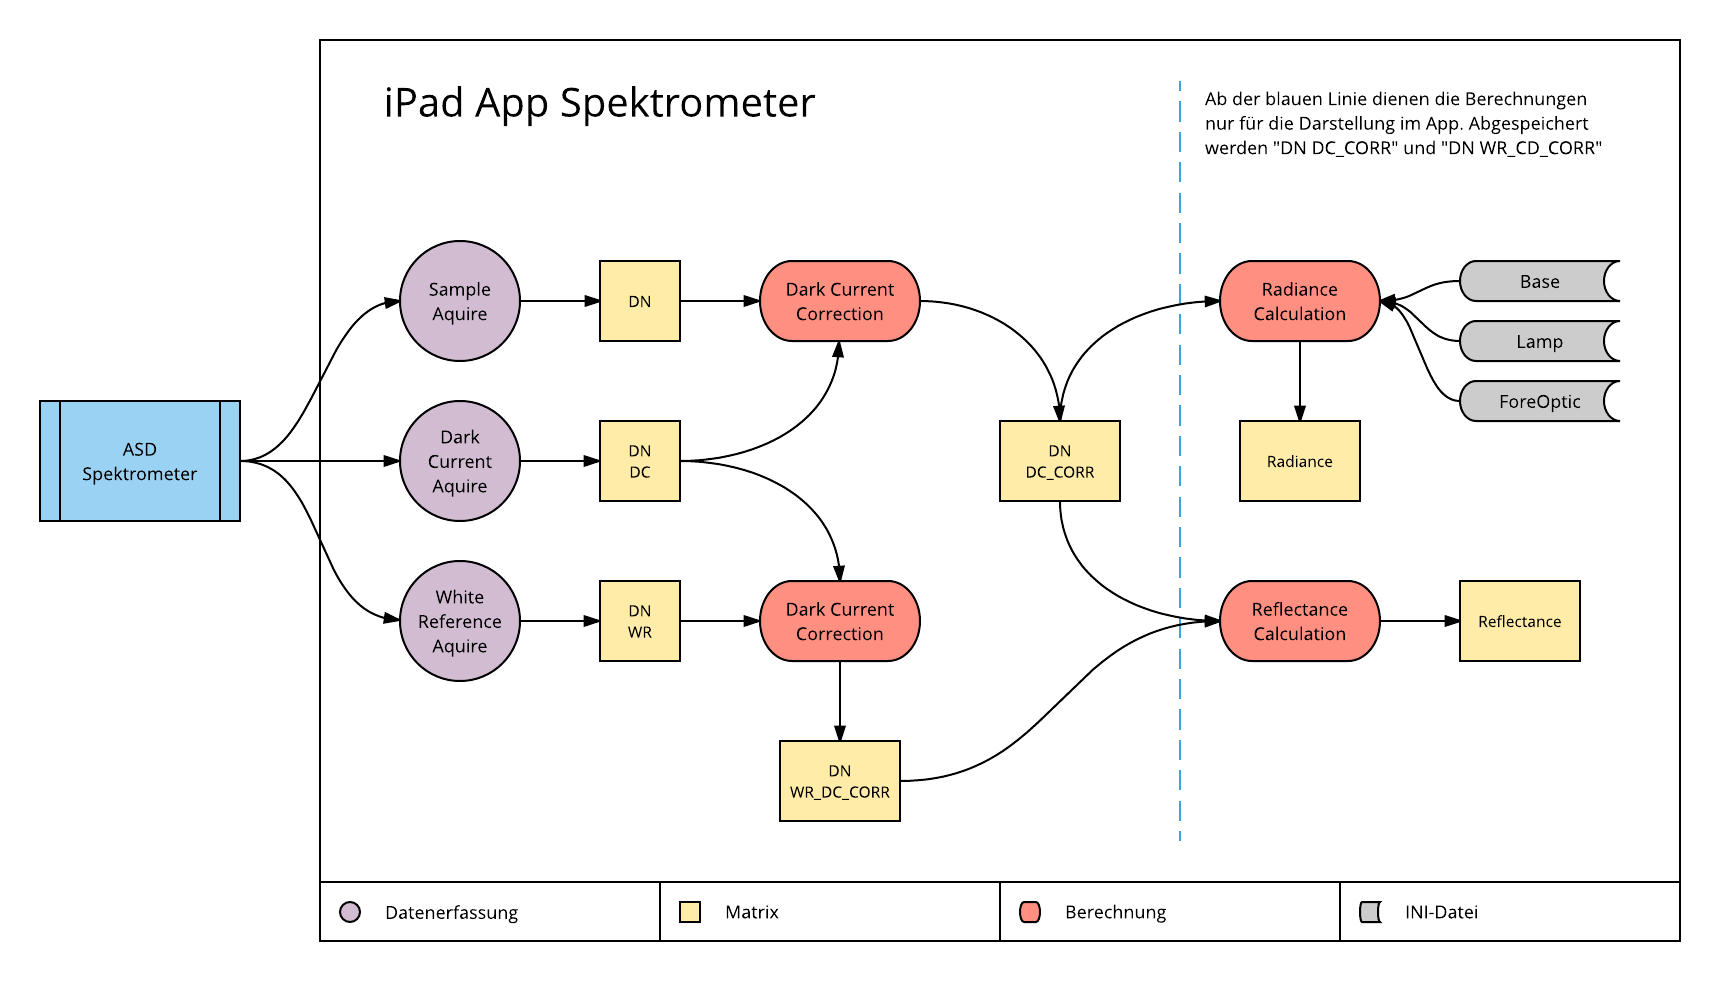
\includegraphics[scale=0.6]{images/Calculations} 
	\caption{Berechnungen f�r Raw, Reflectance und Radiance}
	\label{fig:Calculations}
	\end{center}
\end{figure}

\section{Berechnungen} \label{berechnungen}

\subsection{Dark Current} \label{darkcurrent}
Als Dark Current wird das Spektrum bezeichnet, das gemessen wurde, nachdem dem Spektrometer komplett das Licht genommen wurde. Dies erreicht man auf unterschiedliche Weise. Eine M�glichkeit ist das Kappen der Faser oder das schliessen des mechanischen Shutter. Es gibt bei neueren Ger�ten eine weitere M�glichkeit die Dark Correction mit einer im voraus geladenen Konfigurationsdatei auszuf�hren. Im aktuellen Projekt wird nur die Variante mit dem mechanischen Shutter unterst�tzt.

Die Berechnung wird nur auf den \gls{vnir} Bereich des Spektrums angewendet.

$\forall i \in \{ 0, ... , n \} DC\textsubscript{s}(i) = Ts(i) - Ds(i) + (V\textsubscript{DarkCurrentCorrection} + (T\textsubscript{drift} - D\textsubscript{drift}))$

$n=$ size of the VNIR spectrum \newline
$DCs=$ dark corrected spectrum \newline
$Ts=$ current measured spectrum \newline
$Ds=$ dark measured spectrum \newline
$VDarkCurrentCorrection=$ dark current correction constant\footnote[1]{Dieser Wert wird beim Verbindungsaufbau mit dem Spektrometer ausgelesen und im App zwischengespeichert.} \newline
$Tdrift=$ current measured drift value \newline
$Ddrift=$ dark measured drift value \newline

\subsection{White Reference} \label{whitereference}

\subsection{Radiance} \label{radiance}